\documentclass[11pt,reqno,twoside]{article}

\usepackage{calc}
\usepackage[T1]{fontenc}
\usepackage{times}
\usepackage{lmodern}
%\usepackage{literat}
%\DeclareSymbolFont{operators}{OT1}{\familydefault}{m}{n}
%\addtolength{\textwidth}{-2.2cm} % to emulate the original

\usepackage{amsmath,amssymb,amsfonts}
\usepackage{fullpage}
\usepackage{booktabs}
\usepackage{nicefrac}
\usepackage{siunitx}
\usepackage[numbib]{tocbibind}
\usepackage{wrapfig}
\usepackage[font=small]{caption}
%\usepackage{subcaption}
\usepackage{subfigure}

\usepackage[utf8]{inputenc}
\usepackage{color}
\usepackage{enumitem}
\SetLabelAlign{parright}{\parbox[t]{\labelwidth}{\raggedleft#1}}
\usepackage{psfrag}
\usepackage{amsthm}
\usepackage[english]{babel}
\selectlanguage{english}
%\selectlanguage{catalan}

%\usepackage{eco}
\usepackage[np,autolanguage]{numprint}
  \npdecimalsign{\ensuremath{\cdot}}\npproductsign{\ensuremath{\times}}%
\newcommand{\numold}[1]{\oldstylenums{\numprint{#1}}}

\usepackage{ifpdf}
\usepackage{listings}
\renewcommand{\lstlistingname}{Llistat}

\definecolor{codegreen}{rgb}{0,0.6,0}
\definecolor{codegray}{rgb}{0.5,0.5,0.5}
\definecolor{codepurple}{rgb}{0.58,0,0.82}
\definecolor{backcolour}{rgb}{0.95,0.95,0.92}

%\lstset{language=C, numbers=left, stepnumber=1,
%         basicstyle=\small, numberstyle=\tiny, showspaces=flase}

\lstset{language=matlab,basicstyle=\small}
%, numbers=left, stepnumber=1,
%         basicstyle=\small, numberstyle=\tiny, showspaces=flase}

%\graphicspath{{./figures/}}

%-------------
%pdflatex,
%Macros para producir hyperlinks
\usepackage[pdftex]{graphicx}
\DeclareGraphicsExtensions{.pdf,.jpg,.png,.gif}
\usepackage[pdftex,pagebackref,colorlinks,bookmarksnumbered,
            breaklinks=true,
            colorlinks=true,
            linkcolor=blue,
            citecolor=red,
            urlcolor=magenta]{hyperref}
\hypersetup{
         pdfauthor   = {EquipDocentCalculNumeric},
         pdftitle    = {Template for problems},
         pdfsubject  = {Teaching},
         %pdfpagemode = {FullScreen},
         %pdfstartview = {},
         colorlinks  = {true},
         %bookmarks   = {true},
         %pagebackref = {true},
         bookmarksnumbered = {true},
         %hyperindex  = {true}
}
%\pdfadjustspacing=1
\usepackage{url}

%Disseny de la pàgina
%\usepackage{showframe}
%%%%%%%%%%%%%%%%%%%%%%%%%%%%%%%%%%%%%%%%%%%%%%%%%%%%%%%%%%%%%%%%%%%%%
\usepackage{geometry}
\geometry{
  %papersize={210mm, 296mm},
  a4paper,
  left = 15mm,
  right = 10mm,
  top = 10mm,
  head = 10mm,
  foot = 10mm,
  bottom = 20mm,
  %includeall = false,
}
%%%%%%%%%%%%%%%%%%%%%%%%%%%%%%%%%%%%%%%%%%%%%%%%%%%%%%%%%%%%%%%%%%%%%

\newcommand{\N}{\ensuremath{\mathbb{N}}}
\newcommand{\Z}{\ensuremath{\mathbb{Z}}}
\newcommand{\Q}{\ensuremath{\mathbb{Q}}}
\newcommand{\R}{\ensuremath{\mathbb{R}}}
\newcommand{\C}{\ensuremath{\mathbb{C}}}
\def\ds{\displaystyle}
\def\rme{\mathrm{e}}
\def\rmi{\mathrm{i}}
\def\I{\mathrm{I}}
\def\SVD{\textit{SVD} }
\def\sign{\mathrm{sign}}
\def\diag{\mathrm{diag}}
\def\nuc{\mathrm{Nuc{}}}
\def\rang{\mathrm{Rang{}}}
\def\matlab{
\href{https://es.mathworks.com/products/matlab.html}%
{MATLAB\textsuperscript{\textregistered}}}

\newcommand{\classe}[1]{\ensuremath{\mathcal{C}^{#1}}}
\newcommand{\D}{\ensuremath{\mathcal{D}}}

\newtheorem{thm}{Theorem}[section]
\newtheorem{main_thm}[thm]{Main Theorem}
\newtheorem{cor}[thm]{Corollary}
\newtheorem{lem}[thm]{Lemma}
\newtheorem{prop}[thm]{Proposition}
\newtheorem{defn}[thm]{Definition}
\theoremstyle{remark}
\newtheorem*{rem*}{Remarca}
\newtheorem{rem}{Remarca}%[section]
\newtheorem{nota}{Nota}
\newtheorem{prob}[thm]{Exercici}

\newcommand{\taylor}{\textsf{Taylor} }

\newcommand{\notocsection}[1]{%
    \refstepcounter{section}%
    \section*{\thesection \quad #1}}%

\def\refname{Referències}

\begin{document}
\title{}
\author{}
\date{}
%\maketitle
%\tableofcontents
%\maketitle

\section{Continuation method}\label{sec:pseudoArc} Our goal is to continue
\emph{numerically} a curve $\mathcal{C}\subset\R^{n+1}$, defined
implicitely by the equation
%\begin{displaymath}
       $F(z) = 0$,
%\end{displaymath}
being $F:\R^{n+1}\longrightarrow \R^{n}$ a smooth function. Let us assume
that $z^{j}\in\R^{n+1}$, is a \emph{regular} point of $\mathcal{C}$, so
%\begin{displaymath}
$F\left(z^{j}\right) = 0$, and
  $\mathop{rank}DF\left(z^{j}\right) = n$.
%\end{displaymath}
Moreover, let $v^{j}\in\R^{n+1}$ be an unitary vector tangent to the curve
$\mathcal{C}$ at the point $z^{j}$, $v^{j}\in T_{z^{j}}\mathcal{C}$, so
%\begin{displaymath}
  $\| v^{j}\| = 1$, and
  $DF\left(z^{j}\right) v^{j} = 0$.
%    $\mathcal{C}$ at point $z^{j}$). }
%\end{displaymath}

Then, it is possible to find a new point on the curve,
$z^{j+1}\in\mathcal{C}$, and a new unitary tangent vector, to
$\mathcal{C}$ at $z^{j+1}$, $v^{j+1}\in T_{z^{j+1}}\mathcal{C}$,
$\left\|v^{j+1}\right\| = 1$. If, on its turn, $z^{j+1}$ is a regular point
of $\mathcal{C}$, then  one can look for yet another point on
$\mathcal{C}$, $z^{j+2}\in\mathcal{C}$, and a new unitary tangent vector to
$\mathcal{C}$ at $z^{j+2}$, $v^{j+2}\in T_{z^{j+2}}\mathcal{C}$,
$\left\|v^{j+2}\right\| = 1$, and so on.

Of course, there are several numerical methods to do this
\emph{step-by-step} continuation of $\mathcal{C}$ from an inital point on
the curve, $z^{j}\in\mathcal{C}$, and a (normalizsed) tangent direction at
that point, $v^{j}\in T_{z^{j}}\mathcal{C}$. The one we outline here is the so
called \emph{pseudo-arc continuation method} (see~\cite{Kuznetsov2004},
Chap.~10, Sect.~2, for a complete description). In a nutshell, it consists
in the three stages discussed below.
%\begin{enumerate}[label = \emph{\arabic*.}]
%  \begin{description}
  \paragraph{Stage $1$: Prediction.}
    Take $\hat{z}^{j+1} = z^{j} + h_{j}
    v^{j}\in z^{j} + \left\langle v^{j}\right\rangle$ as an approximation
    for another new point $z^{j+1}\in\mathcal{C}$. Here $h_{j} > 0$ is the
    pseudo-arc length, and can be conveniently adapted at each step.
%%
  \paragraph{Stage $2$: Correcton.}
 Refine the approximation $\hat{z}^{j+1}$ to
    find $z^{j+1}\in\R^{n+1}$ such that $F\left(z^{j+1}\right) = 0$.
    However, as the system $F(z) = 0$ has $n$ equations and $n+1$ unknowns
    $z_{1}, z_{2},\dots,z_{n},z_{n+1}$, we need to ask for an additional
    condition: in particular, we shall require that
    $z^{j+1}\in\hat{z}^{j+1} +\left\langle v^{j}\right\rangle^{\perp}$, i.e., that
    $z^{j+1}$ belongs to
    the hyperplane orthogonal to the vector $v^{j}$ that holds
    $\hat{z}^{j+1}$
    (see Figure~\ref{fig:pseudo-arc}). The
    corresponding equation con be formulated as
    \begin{align*}
      \left\langle v^{j}, z^{j+1} - \hat{z}^{j+1}\right\rangle &=
      \left\langle v^{j}, z^{j+1} - z^{j} - h_{j} v^{j}\right\rangle \\
      &= \left\langle v^{j}, z^{j+1}\right\rangle -
        \left\langle v^{j}, z^{j}\right\rangle -
        h_{j} \left\langle v^{j}, v^{j}\right\rangle\\
      &=  \left\langle v^{j}, z^{j+1}\right\rangle -
          \left\langle v^{j}, z^{j}\right\rangle - h_{j} = 0,
    \end{align*}
    where $\langle\cdot, \cdot\rangle$ stands for the \emph{inner} (or dot)
    product $\left\langle\xi, \eta\right\rangle := \xi_{1}\eta_{1} + \dots +
    \xi_{m}\eta_{m}$, $\xi, \eta\in\R^{m}$. Hence $z^{j+1}$ will be
    given by the solution of the nonlinear system,
    \begin{displaymath}
      \begin{split}%\label{eq:enlarged-system-corrector}
        F(z) &= 0,\\
        \left\langle v^{j}, z\right\rangle &= \left\langle v^{j},
        z^{j}\right\rangle - h_{j}
        \end{split}
    \end{displaymath}
    that can be solved by some iterative method (for example, Newton
    method) taking as initial approximation. $z^{(0)} = \hat{z}^{j+1}$.
  %
\paragraph{Stage $3$: Tangent vector.} To find the tangent vector to the
curve at the new point $z^{j+1}\in\mathcal{C}$ found at Stage
$2$, $v^{j+1}\in  T_{z^{j+1}}\mathcal{C}$, first we solve the
$(n+1)$-dimensional linear system
    \begin{equation}\label{eq:appended-system}
      \begin{split}
      DF\left(z^{j+1}\right)v &= 0,\\
      \left\langle v^{j}, v \right\rangle &= 1.
    \end{split}
  \end{equation}
  As it is pointed out in~\cite{Kuznetsov2004}:
  \begin{enumerate}[label = \emph{(\roman*)}]
    \item If $\mathcal{C}$ is a regular curve and $z^{j}$, $z^{j+1}$ are close
  enough, the system~\eqref{eq:appended-system} is nonsingular.
    \item The solution, $v^{\ast}\in\R^{n+1}$,
  of~\eqref{eq:appended-system} satisfies $\left\langle v^{j},
  v^{\ast}\right\rangle = 1$, so the direction along the curve is
  preserved.
\end{enumerate}
Next, we normalize. If $v^{\ast}\in\R^{n+1}$ denotes the solution
of~\eqref{eq:appended-system}, we divide by its norm, so $v^{j+1} =
v^{\ast}/\left\|v^{\ast}\right\|$. This is the tangent vector we look for.
\hfill $\diamondsuit$
%\end{description}

\begin{figure}[!t]
  \centering
  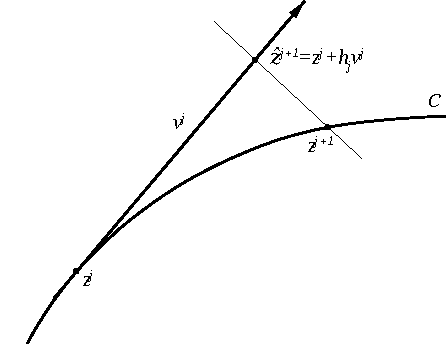
\includegraphics[scale=1.0]{arcstep}
  \caption{We add an extra condition: $z^{j+1}\in
  \hat{z}^{ji+1} + \left\langle v^{j}\right\rangle^{\perp}$.
See~\cite{Kuznetsov2004}, Figure 10.6(b).\label{fig:pseudo-arc}}
\end{figure}

Now, the process can be iterated using the output of Stage $3$, the tangent
vector $v^{j+1}$ to feed Stage $1$ and find a another point close to the
curve  $\mathcal{C}$, and so on. If for the new computed point curve $C$,
and so on. If at Stage $2$, $\mathop{Rank} DF\left(z^{k}\right) < n$, for
the new computed point, $z^{k}\in\mathcal{C}$, then
 one has to stop the process and analyse for the possible
appearing of branches (bifurcations).

Neverteless, to start the process we need an initial point on the curve and
its corresponding tangent vector, $z^{0}\in\mathcal{C}$ and $v^{0}\in
T_{z^{0}}$. To find $z^{0}$ we can proceed as follows: let us assume that
we have an approximation for the initial solution, $\hat{z}^{0} =
\left(\hat{z}^{0}_{1},\dots,\hat{z}^{0}_{n}, \hat{z}^{0}_{n+1}\right)$,
then we fix one of its components, suppose that we take the last one,
$\hat{z}^{0}_{n+1}$ and solve the $n$-dimensional system,

\begin{displaymath}
  \begin{array}{rcl}
    F_{1}\left(z_{1},\dots, z_{n+1},
    \hat{z}^{0}_{n+1}\right)&\!\!\!=&\!\!\! 0,\\
    F_{2}\left(z_{1},\dots, z_{n+1},
  \hat{z}^{0}_{n+1}\right)&\!\!\!=&\!\!\! 0,\\ 
  \hdotsfor{3}\\ 
    F_{n}\left(z_{1},\dots, z_{n+1},
  \hat{z}^{0}_{n+1}\right)&\!\!\!=&\!\!\! 0, 
\end{array}
\end{displaymath}
by the Newton method, starting with $z_{1} = \hat{z}^{0}_{1},\dots,z_{n} =
\hat{z}^{0}_{n}$. If the method converges, we have an initial point on the
curve, $z^{0} = \left(z^{0}_{1},\dots,z^{0}_{n},\hat{z}^{0}_{n+1}\right)$.
Besides, to 

\bibliographystyle{plain}
\bibliography{references}
%\nocite{*}
\end{document}

%%% Local Variables:
%%% mode: latex
%%% TeX-master: "manual"
%%% End:
